\documentclass[preprint]{sigplanconf}

\usepackage{amsmath}
\usepackage{listings}
\usepackage{float}
\usepackage{graphicx}
\usepackage{adjustbox}
\usepackage{multirow}
\usepackage{color}


\newcommand{\lyxdot}{.}

\floatstyle{ruled}
\newfloat{Listing}{tbp}{loa}

\begin{document}

\special{papersize=8.5in,11in}
\setlength{\pdfpageheight}{\paperheight}
\setlength{\pdfpagewidth}{\paperwidth}

\conferenceinfo{CONF 'yy}{Month d--d, 20yy, City, ST, Country} 
\copyrightyear{20yy} 
\copyrightdata{978-1-nnnn-nnnn-n/yy/mm} 
\doi{nnnnnnn.nnnnnnn}

% Uncomment one of the following two, if you are not going for the 
% traditional copyright transfer agreement.

%\exclusivelicense                % ACM gets exclusive license to publish, 
                                  % you retain copyright

%\permissiontopublish             % ACM gets nonexclusive license to publish
                                  % (paid open-access papers, 
                                  % short abstracts)

\titlebanner{banner above paper title}        % These are ignored unless
\preprintfooter{short description of paper}   % 'preprint' option specified.

\title{Understanding Which Factors Influence the Choice for a Typing System}

\authorinfo{Carlos Souza}
           {Federal University of Minas Gerais}
           {carlosgsouza@gmail.com}
\authorinfo{Eduardo Figueiredo}
           {Federal University of Minas Gerais}
           {figureido@dcc.ufmg.br}
\authorinfo{Marco Túlio Valente}
           {Federal University of Minas Gerais}
           {mtov@dcc.ufmg.br}

\maketitle

\begin{abstract}
One of the most important things to be taken into account when choosing a programming language is its typing system, static or dynamic. 
This question has become increasingly more important due to the recent popularization of dynamic languages such as Ruby and JavaScript. 
This paper studies which are the most influencing factors for a programmer when choosing between typing systems. 
An analysis of the source code of over seven thousand projects written in Groovy, a programming language where one can mix static and dynamic typing freely, shows in which situations programmers prefer a typing system over the other. 
Results of this study suggest that the previous experience of the programmer, project size, complexity of modules, scope and visibility of statements are some of the most important factors in this decision.
\end{abstract}

\category{CR-number}{subcategory}{third-level}

% general terms are not compulsory anymore, 
% you may leave them out
\terms
term1, term2

\keywords
keyword1, keyword2

\section{Introduction}
When choosing a programming language for a project, a developer must consider several characteristics of that language.
One of the most important is its typing system.
This, which can be static or dynamic, determines when the type of a statement should be defined\cite{types_and_programming_languages}. 
Statically typed languages, such as Java and C\#, require the type of a statement to be defined by the programmer, which can then be used by the compiler to check for any typing errors. 
On the other side, in dynamically typed languages, like Ruby and JavaScript, the definition of the type of a statement only happens during run time.

The discussion about what is the best typing system has become increasingly more important in recent years due to rapid popularization of dynamically typed languages. 
According to The TIOBE Programming Community Index \cite{tiobe}, a well-known ranking that measures the popularity of programming languages, 27\% of the programming languages in the industry are dynamically typed. 
In 2001, this number was only 17\%. 
Among the 10 languages on top of the ranking, four are dynamically typed: JavaScript, Perl, Python and PHP. 
In 1998, none of these languages was among the top 10 ranking.

Several factors may be considered when choosing betwen a dynamcally or statically typed language. 
Since dynamically typed languages are simpler, they allow programmers to perform their tasks more quickly \cite{types_and_programming_languages} and adapt to changin requirements \cite{gradual_typing}.
Also, by removing the repetitive work of defining types, these languages allow their users to focus on the problem to be solved rather than spending time with the rules of the language \cite{dynamically_typed_languages}.

Statically type languages also have their advantages. 
These allow compilers to look for type errors \cite{should_your_specification_language_be_typed}. 
Typed declarations increase the maintainability of systems because they document the code, informing the programmer the nature of each variable \cite{type_systems,mayer2012static}. 
Systems built with these languages tend to be more efficient since they do not need to perform type checking during their execution \cite{bruce2002foundations,jit}. 
Finally, modern development environments, such as Eclipse and IDEA, are able to assist programmers with functionalities such as code completion based the information
they get from statically typed declarations \cite{bruch2009learning}.

This paper presents a study aiming to understand which factors actually influence the decision of a developer for typing their declarations or not. 
This question was studied based on the analysis of a massive dataset with more than seven thousand projects.
These projects were written in Groovy, a language with a hybrid typing system which allows developers to choose, for each statement, either to type or not.
Through a static analysis of these projects, it was possible to understand when developers choose each type system and then extract what are the factors that influence this decision.

The remainder of this paper is organized as follows. 
Section \ref{sec:A-Linguagem-Groovy} introduces the main concepts of the Groovy program language. 
Sections \ref{sec:Configura=0000E7=0000E3o-do-Estudo} and \ref{sec:Resultados} describe the configuration of the study and its results. 
Section \ref{sec:ameaca} discusses threatens to validity and section \ref{sec:Trabalhos-Relacionados} shows related work. 
Finally, section  \ref{sec:Conclus=0000E3o-e-Trabalhos} concludes this study and suggests future works.















%
%  THE GROOVY LANGUAGE
%

\section{The Groovy Language\label{sec:A-Linguagem-Groovy}}
Groovy is an object-oriented programming language designed to run on the Java Virtual Machine.
It builds upon the strengths of Java, but has additional features inspired by dynamic languages such as Python and Ruby.
Its adoption has grown remarkably over the last years, specially among Java developers who seek more dynamism without having to learn a completelly new language.
Groovy allows programmers to use both static and dynamic type systems, which makes it ideal for a comparative study between those two type systems.

Despite having been launched less than ten years ago, Groovy is already a very popular language.
According to the Tiobe Programming Index, Groovy is the 22\textsuperscript{st} most popular language in the software industry\cite{tiobe}, ahead of languages like Prolog, Haskell and Scala. 

The syntax of the Groovy language is similar to Java's and most of Java syntax is also valid in Groovy.
Like Java, Groovy code is compiled to bytecode, allowing it to seamlessly integrate with existing Java classes and libraries. 
These factors have attracted a large number of Java programmers who want to use Groovy's dynamic functionality without having to learn a completely different language or change the execution platform of their systems. 

Groovy was designed to be more expressive and concise than Java.
Below we show two implementations of a simple algorithm.
Given a list of numbers, return a list with the even numbers of that list.
Listing \ref{javaClass} shows the Java implementation while Listing \ref{groovyClass} shows the Groovy counterpart. 
Note that Groovy supports lists nativelly(lines 3, 6 and 14) and operator overloading (line 6).


Many of the boilerplate elements from Java aren't required in Groovy.  
As shown in Listing \ref{groovyClass}, semicolons are optional, except when there are multiple statements in the same line. 
When the keyword $return$ is omitted (line 10), the last expression evaluated with a method is returned. 
Also, parenthesis in method calls can often be omitted (line 16).
In addition to that, frequently used classes like those of the $java.util$ package are imported by default and thus don't need to be implicitly imported.
Least, Groovy provides easy access to frequently used methos such as $System.out.println$ (line 16). Other important 

% This gives much more expressiveness to a programmer for common tasks that would rather require more boilerplate code in Java.
% All in all ... Compared to Listing \ref{javaClass}, Groovy code can be much more expressive.

\begin{Listing}[ht]
\begin{lstlisting}[language=Java,tabsize=2,breaklines=true,numbers=left]
import java.util.ArrayList;
import java.util.List;

public class JavaFilter {
	List<Integer> evenNumbers(List<Integer> list) {
		List<Integer> result = new ArrayList<Integer>();
		for(int item : list) {
			if(item % 2 == 0) {
				result.add(item);
			}
		}

		return result;
	}

	public static void main(String[] args) {
		List<Integer> list = new ArrayList<Integer>();
		list.add(1);
		list.add(2);
		list.add(3);
		list.add(4);

		List<Integer> result = new JavaFilter().evenNumbers(list);
		System.out.println(result);
	}
}
\end{lstlisting}
\caption{A simple algorithm written in Java}
\label{javaClass}
\end{Listing}

\begin{Listing}[ht]
\begin{lstlisting}[language=Java,tabsize=2,breaklines=true,numbers=left]
class GroovyFilter {
	List<Integer> evenNumbers(List<Integer> list) {
		List<Integer> result = []
		for(int item : list) {
			if(item % 2 == 0) {
				result << item
			}
		}

		result
	}

	public static void main(String[] args) {
		List<Integer> list = [1, 2, 3, 4]
		List<Integer> result = new GroovyFilter().evenNumbers(list)
		println result
	}
}
\end{lstlisting}
\caption{A simple algorithm written in Groovy}
\label{groovyClass}
\end{Listing}

Groovy's design was influenced by dynamic feature of programming languges like Ruby and Python.
Listing \ref{dynamicInfuence} shows how these features can be used to rewrite the same algorithm presented in Listing \ref{javaClass} in a single line of code. 
This code snippet makes use of closures to allow a programmer to define a filter logic for the method $findAll$.
This allows a functional programming style of code which allows a high level of expressivenes for the programmer.
Notice that this is a script, rather than a class, and thus the programmer doesn't have to write class.

\begin{Listing}[ht]
\begin{lstlisting}[language=Java,tabsize=2,breaklines=true]
println([1, 2, 3, 4].findAll {it % 2 == 0})
\end{lstlisting}
\caption{A class written in Groovy}
\label{dynamicInfuence}
\end{Listing}

Metaprogramming is another dynamic feature present in Groovy. 
Listing \ref{metaprogramming} shows how to add a method to an existing class dynamically.
By adding the method $evenNumbers()$ to the $List$ class, it is possible to achieve higher expressivenes.
This is specially useful when implementing Domain Specific Languages.

\begin{Listing}[ht]
\begin{lstlisting}[language=Java,tabsize=2,breaklines=true,numbers=left]
List.metaClass.evenNumbers = {
	delegate.findAll {it % 2 == 0}
}
println([1, 2, 3, 4].evenNumbers())

\end{lstlisting}
\caption{An example of metaprogramming in Groovy}
\label{metaprogramming}
\end{Listing}

When Groovy 1.0 was first launched, in 2007, it was a purelly dynamically typed language.
However, it allowed programmers to optionally type their statements.
This is illustrated in Listing \ref{dynamicTyping}. 
It shows examples of declarations of typed and untyped methods, fields and variables combined flexibly in the same class.


\begin{Listing}[ht]
\begin{lstlisting}[language=Java,tabsize=2,breaklines=true,numbers=left]
class DynamicTyping {
	private String typedField
	private untypedField

	DynamicTyping(untypedParam, String typedParam) {}

	def untypedMethod(untypedParam, int typedParam) {
		def untypedVariable = untypedParam + typedParam
		return result
	}

	int typedMethod()  {
		String typedVariable = ""
		return typedVariable
	}
}
\end{lstlisting}
\caption{Groovy is a dynamic language}
\label{dynamicTyping}
\end{Listing}

This kind of typing shown in Listing \ref{dynamicTyping} should not be confused with static typing.
Groovy compiler still isn't able to check type correctness.
For example, the snippet of code shown in Listing \ref{typeError} compiles without any errors, but fails during execution with a type error.

\begin{Listing}[ht]
\begin{lstlisting}[language=Java,tabsize=2,breaklines=true]
int integer = "string"
\end{lstlisting}
\caption{A class written in Groovy}
\label{typeError}
\end{Listing}

Since Groovy 2.0, Groovy allows programmers to explicitly activate static typing with the usage of the $@TypeChecked$ annotation.
In this mode, the Groovy compiler will look for type errors and fail compilation if it finds any.
Listing \ref{staticTyping} shows a class with the $@TypeChecked$.
When this class is compiled, the compiler fails with a compilation error since the method $sum$ is supposed to receive to parameters with the type $int$, but is called with two parameters of the type $String$.
%% TODO: Talk about gradual type systems \cite{gray05,gray08,gray11,siek07,takikawa12}

\begin{Listing}[ht]
\begin{lstlisting}[language=Java,tabsize=2,breaklines=true,numbers=left]
@TypeChecked
class TypeCheckedGroovyClass {
	
	static int sum(int a, int b) {
		a + b
	}

	public static void main(String[] args) {
		println sum("1", "2")
	}
}
\end{lstlisting}
\caption{A class written in Groovy}
\label{staticTyping}
\end{Listing}

The $@TypeChecked$ annotation is reasonably recent and most Groovy programmers still don't use. 
Typing annotations on the other side are very popular.
Although they don't provide static type checking, they are capable of documenting the code and aiding in the integration with development tools.

\section{Study Setup\label{sec:Configura=0000E7=0000E3o-do-Estudo}}
TODO: Right now I only have the static code analyzer here. I will refactor this section so I can list all the phases of my study. It's still not clear where I can describe this static code analyzer though.

\subsection{Static Code Analyzer}
The static code analyzer used in this work is based on the Groovy metaprogramming library. 
With this library, it's possible to create an abstract syntax tree (AST) from Groovy source code using one of the various stages of the Groovy compiler.
The phase chosen for this analysis was the conversion phase, which has sufficient information to determine the type system of each statement.
It occurs before the compiler tries to resolve any external dependencies, making it possible to analyze each file separately without having to compile the whole project.

The static code analyzer is capable of analyzing the following types of statements
\begin{itemize}
	\item Return Methods
	\item Method Parameters
	\item Constructor Parameters
	\item Fields
	\item Local Variables
\end{itemize}

For each item listed above, it is possible to answer the following questions
\begin{itemize}
	\item What is the typing system of the statement?
	\item Is the statement part of a script or a class?
	\item Is the statement part of a test class?
	\item What is the visibility of the statement? (except for local variables)
\end{itemize}





\section{Dataset\label{sec:dataset}}
TODO: This is also just the VEM version. The purpose of this section is to present data about my dataset that is fundamental for my discussion. Also, I believe that having a dedicated section to my dataset is a good idea as it highlights one of the strong points of this article.

The projects used in this study were obtained from GitHub, a popular source control service based on Git.
Using Github API, it was possible to obtain the source code of 7268 projects with a total of 9.8 million lines of code. 
The distribution of the size of these designs is shown in figure \ref{fig:size_distribution}. 
These projects were developed by a total of 4806 developers and, together, they have approximately 169 thousand Groovy files.

\begin{figure}[ht]
\centering 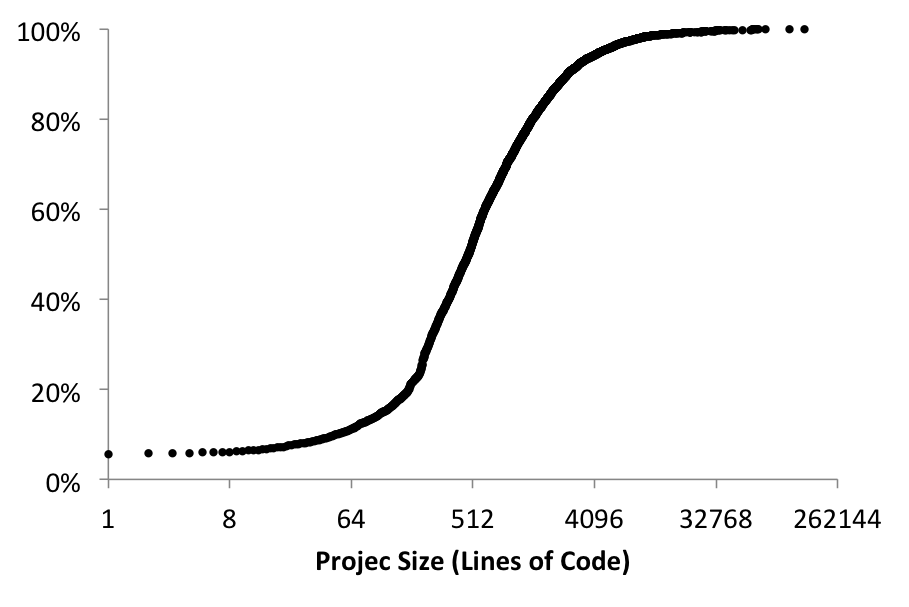
\includegraphics[width=0.45\textwidth]{images/size_distribution}
\caption{Project Size Distribution}
\label{fig:size_distribution} 
\end{figure}

\begin{figure}[ht]
\centering 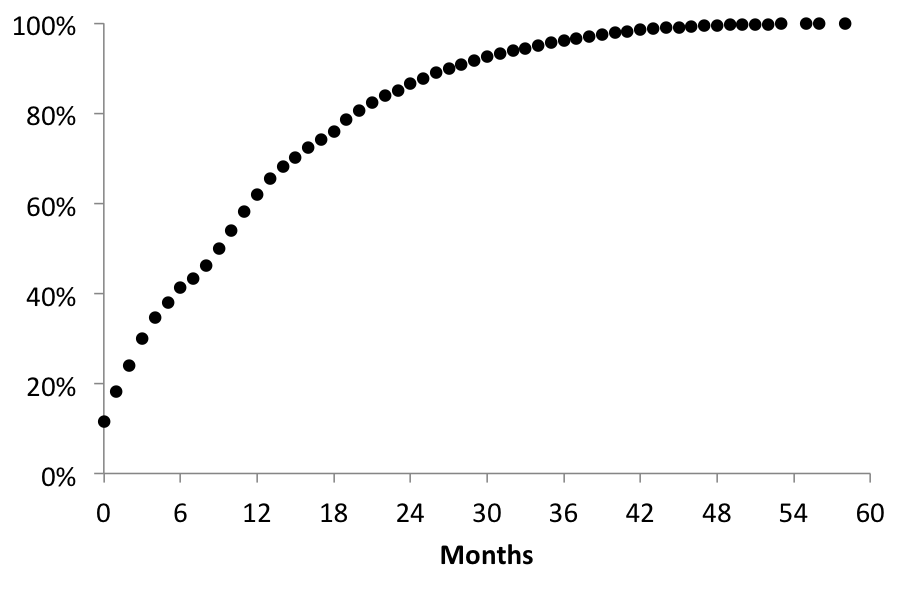
\includegraphics[width=0.45\textwidth]{images/age_distribution}
\caption{Project Age Distribution}
\label{fig:age_distribution} 
\end{figure}
 
\begin{table}[ht]
\caption{Distribution of the Number of Developers}


\centering{}%
\begin{tabular}{|c|c|c|}
\hline 
Number of Developers & Fraction of Projects\tabularnewline
\hline 
\hline 
1 & 84\% \%\tabularnewline
\hline 
2 & 9\% \%\tabularnewline
\hline 
3 & 3\% \%\tabularnewline
\hline 
4 or more & 4\% \%\tabularnewline
\hline 
\end{tabular}
\label{tab:number_of_developers}
\end{table}






\section{Results\label{sec:Resultados}}

In this section we present the results of the analysis of the declarations of the projects described in section \ref{sec:dataset}. 
These results will be discussed in more details in section \ref{sec:Discussion}.

\subsection{Overall Result\label{sub:overall-result}}
The analysis shows that 61\% of the statements are typed, while only 39\% of these are dynamically typed. This results considers all declarations of the 7268 projects in the dataset.


\subsection{Results by Declaration Type\label{sub:declaration-type-results}}
Figure \ref{fig:tipo_declaracao} shows the amount of typed and untyped declarations for each type of declaration. 
Untyped declarations are far more frequent in local variables that in other types of statements.
Fields, method returns and parameters on the other side are mostly typed. In particular, constructor parameters are typed in more than $90\%$ of the declarations.

\begin{figure}[ht]
\centering 
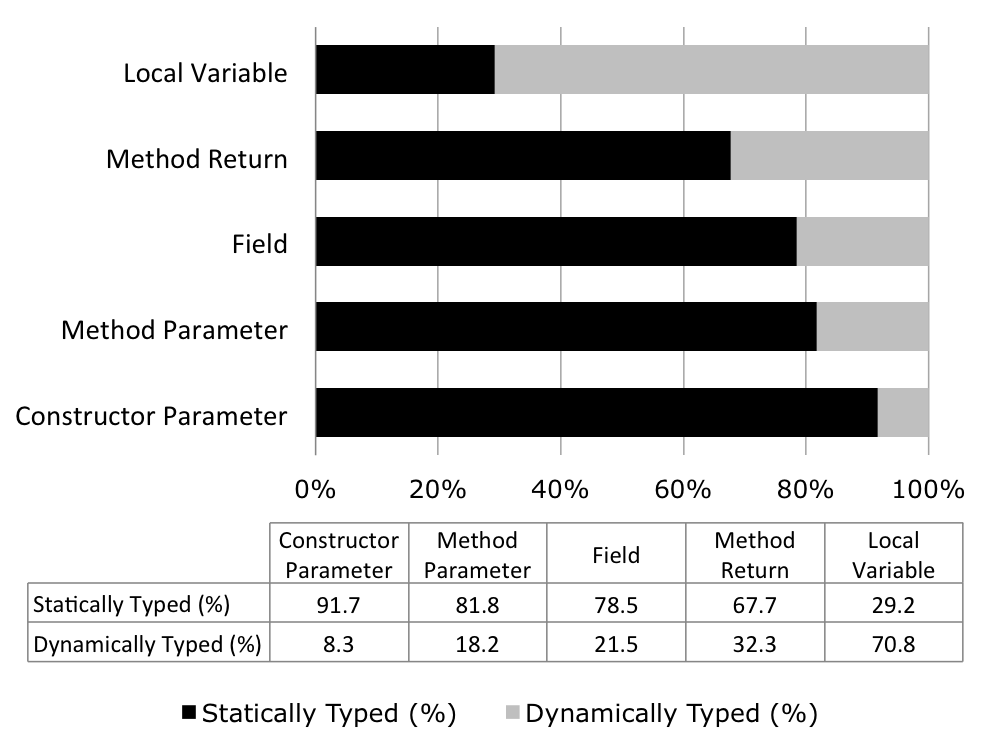
\includegraphics[width=0.45\textwidth]{images/tipo} 
\caption{Type Systems by Declaration Type.}
\label{fig:tipo_declaracao} 
\end{figure}

\subsection{Results by Visibility\label{sub:visibility-results}}
In this section, we break down the results shown above by visibility. Our goal is to understand if the visibility of the declarations have any sort of influence on the choice for using types or not.

Figure \ref{fig:method_return_visibility} shows that there is little difference between the use of types in declarations of the return of private and public methods. 
With $64.44\%$ and $67.26\%$ typed declarations respectively, these results don't present any significant divergence from the overall results shown in section \ref{sec:Resultados}.
On the other side, the return of protected methods, are almost always typed.

\begin{figure}[ht]
\centering 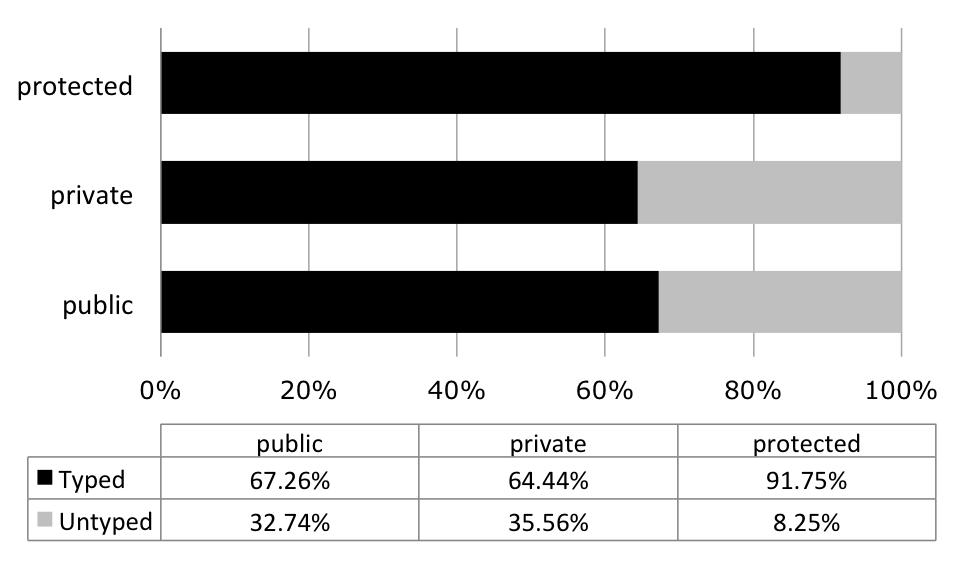
\includegraphics[width=0.45\textwidth]{images/method_return_visibility} 
\caption{Type Systems by Declaration Visibility}
\label{fig:method_return_visibility} 
\end{figure}

Figure \ref{fig:method_parameter_visibility} shows the results of the analysis of method parameter declarations. 
Compared to the results for method returns shown in figure \ref{fig:method_return_visibility}, parameters of public methods are typed more often.
While public method returns have types in $67.26\%$ of the times, public method parameters have more than $80\%$ their declarations typed.

\begin{figure}[ht]
\centering 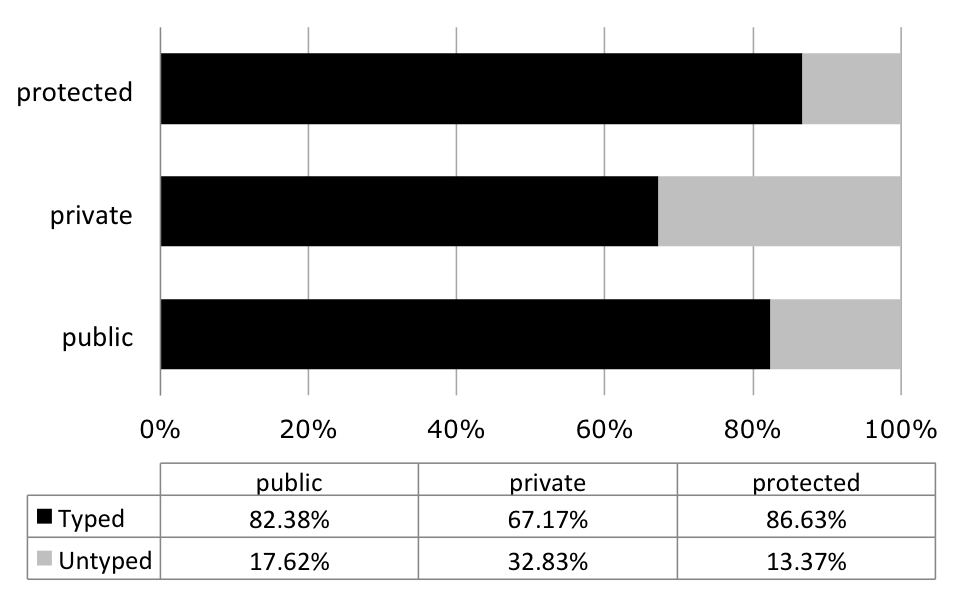
\includegraphics[width=0.45\textwidth]{images/method_parameter_visibility} 
\caption{Type Systems by Declaration Visibility}
\label{fig:method_parameter_visibility} 
\end{figure}

Results for constructor parameters are shown in figure \ref{fig:constructor_parameter_visibility}.
These results are close to the results observed for non-constructor method parameters above. 

\begin{figure}[ht]
\centering 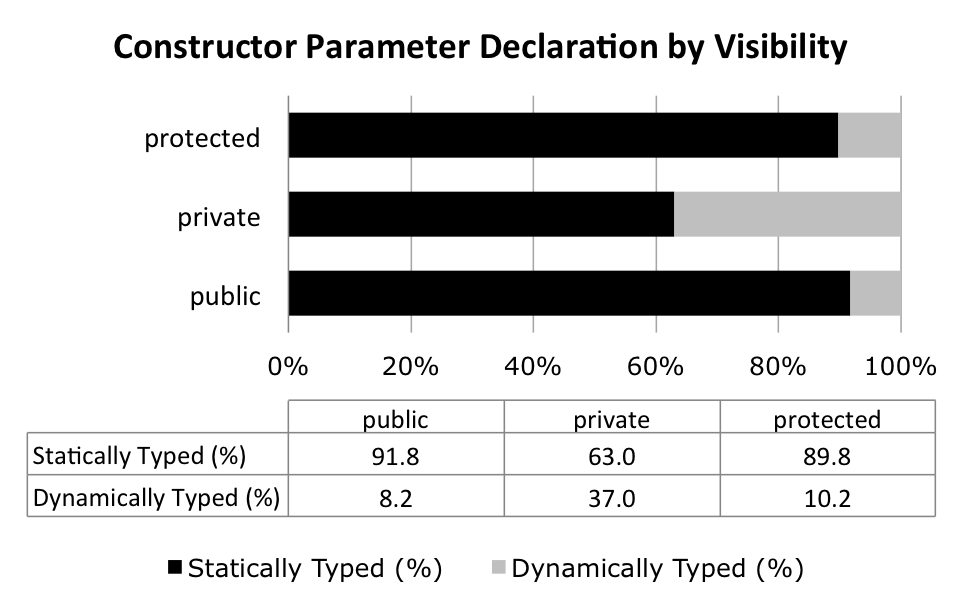
\includegraphics[width=0.45\textwidth]{images/constructor_parameter_visibility} 
\caption{Type Systems by Declaration Visibility}
\label{fig:constructor_parameter_visibility} 
\end{figure}


Figure \ref{fig:field_visibility} shows the results for field declarations. 
Different from previous analyzed declarations, protected fields are significantly less typed than public fields. 
While the first is typed in $88.8\%$ of the cases, $80.5\%$ of the latter are typed.
Another difference is that private fields are slightly more typed than other private declarations.
While this frequency is $72.4\%$ for private fields, method returns, method parameters and constructor parameters don't get typed more than $67\%$ of the time.


\begin{figure}[ht]
\centering 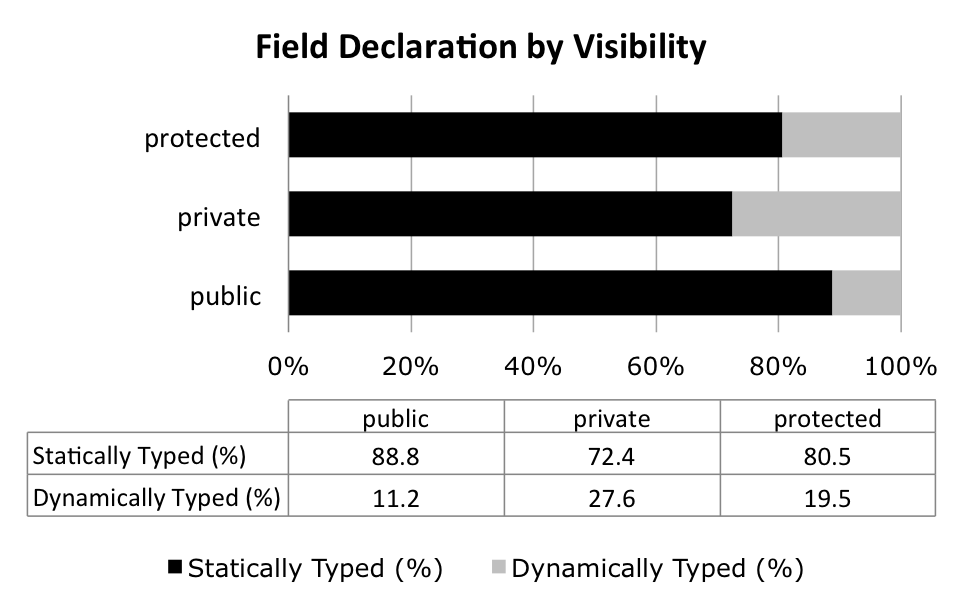
\includegraphics[width=0.45\textwidth]{images/field_visibility} 
\caption{Type Systems by Declaration Visibility}
\label{fig:field_visibility} 
\end{figure}

In summary, for all types of declarations, private declarations are less typed than public and protected.
Protected declarations, on the other side, are usually those typed in most cases. The only exception to this are fields, where the usage of types in public declarations surpasses those of protected declarations by $8\%$.

\subsection{Results by Project Size\label{sub:size-results}}
In this section we show how the use of types in declarations varies according to the project size. 
The goal of this analysis is to understand if there is any correlation between the usage of types and the complexity of software projects. 

Project size is a means to measure the complexity of a project.
Usually, the larger the project, the greater the difficulty of integration and the need for maintenance. 
There are metrics far more effective for this purpose such as [TODO].
This simple approach is very useful in a study such as this because it doesn't require the source code to be compiled to determine the project complexity. 
Requiring projects to be compiled would drastically limit the number of projects

Results are shown for public, private and protected method returns (figures \ref{fig:size_pubMethodReturn}, \ref{fig:size_priMethodReturn}, \ref{fig:size_proMethodReturn} respectively). 
We also show results for local variables (figure \ref{fig_size_localVariable}). 
Results for other types of declarations were omitted due to lack of space.
The behavior for these other declarations is described in table \ref{tab:size_dynamic_spearman}, which shows the spearman ranking for the relation between size and dynamic typing for each type of declaration considered in this study.

In the graphs below, each bar shows the average use of dynamically typed declarations of projects grouped by their size.
The boundaries of each group are defined under each bar.
For example, a project with $1500$ lines of code is in the fifth group, since $1500$ lies within the interval $]1024, 2048]$.
Notice that we are using a logarithm scale for the project size in these graphs. (TODO explain why)

The usage of untyped declarations of public method returns decreases with the project size.
While projects with less than $1024$ lines of code have almost $40\%$ of their declarations untyped, this number is less than $20\%$ in project with over $65536$ lines of code.

\begin{figure*}[ht]
\centering 
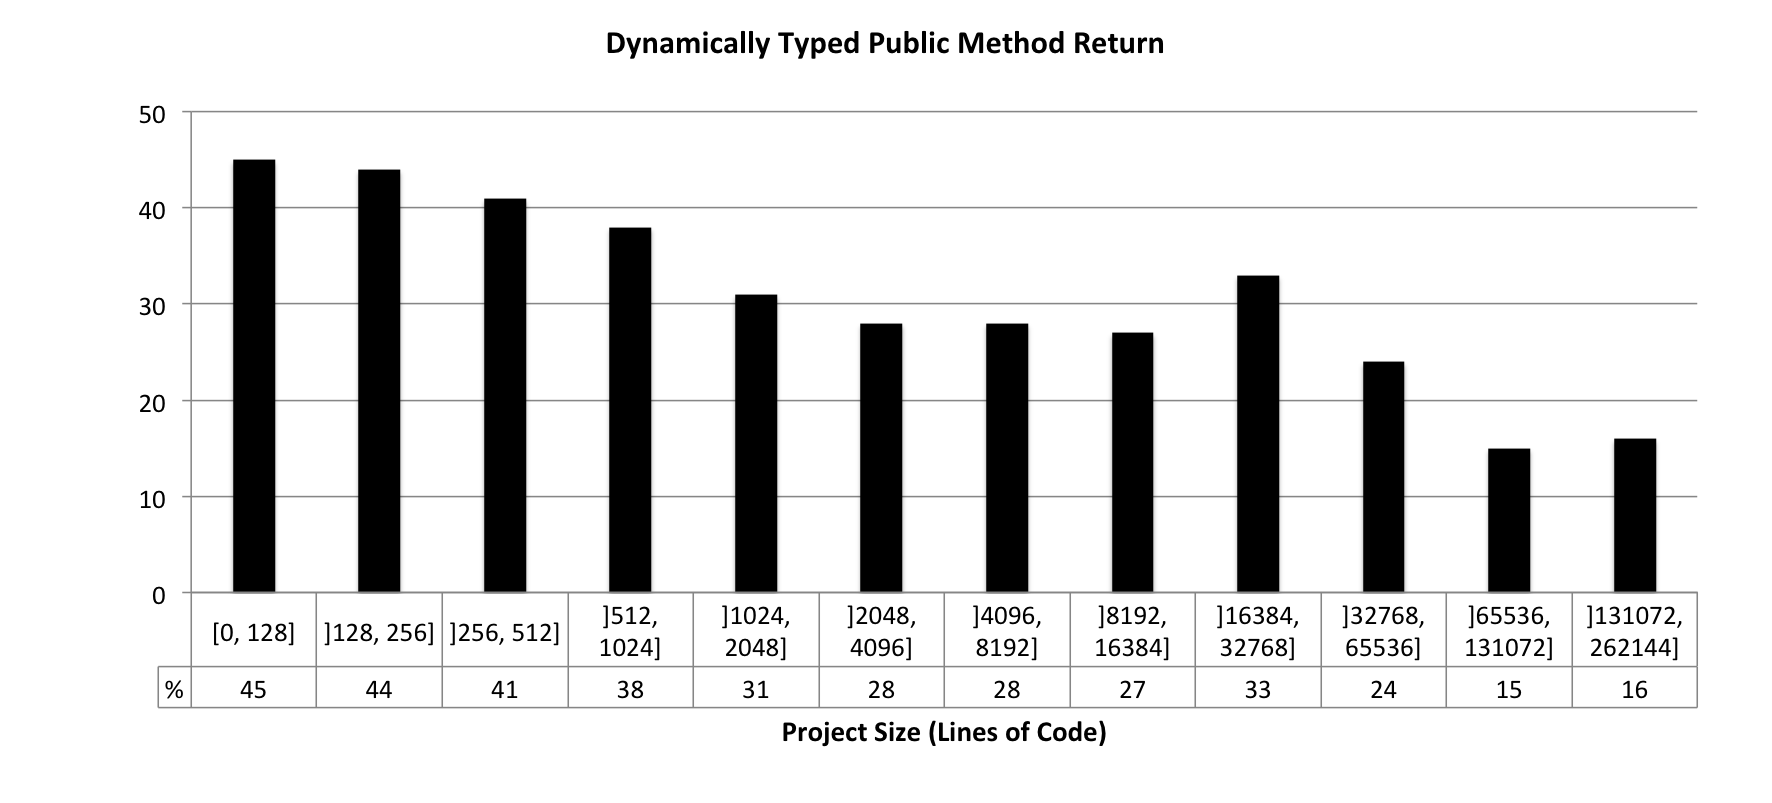
\includegraphics[width=1\textwidth]{images/size_pubMethodReturn} 
\caption{Dynamic Typing usage in local variables}
\label{fig:size_pubMethodReturn} 
\end{figure*}

Figures \ref{fig:size_priMethodReturn}) and \ref{fig:size_proMethodReturn}) show that, different from public method returns, private and protected method returns have no correlation with the project size.

\begin{figure*}[ht]
\centering 
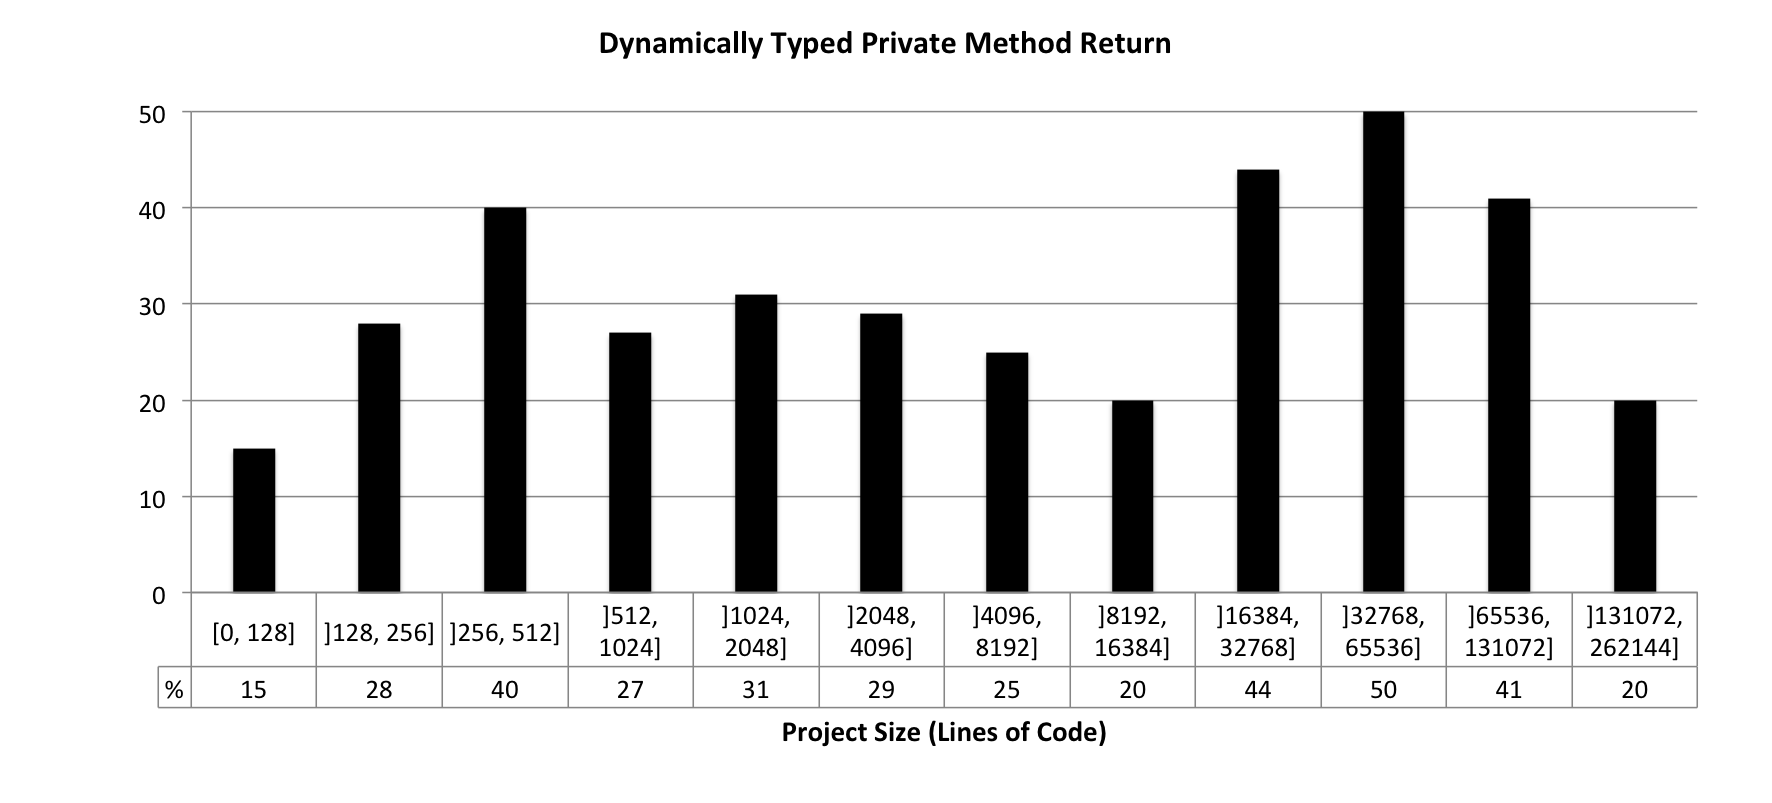
\includegraphics[width=1\textwidth]{images/size_priMethodReturn} 
\caption{Dynamic Typing usage in local variables}
\label{fig:size_priMethodReturn} 
\end{figure*}

\begin{figure*}[ht]
\centering 
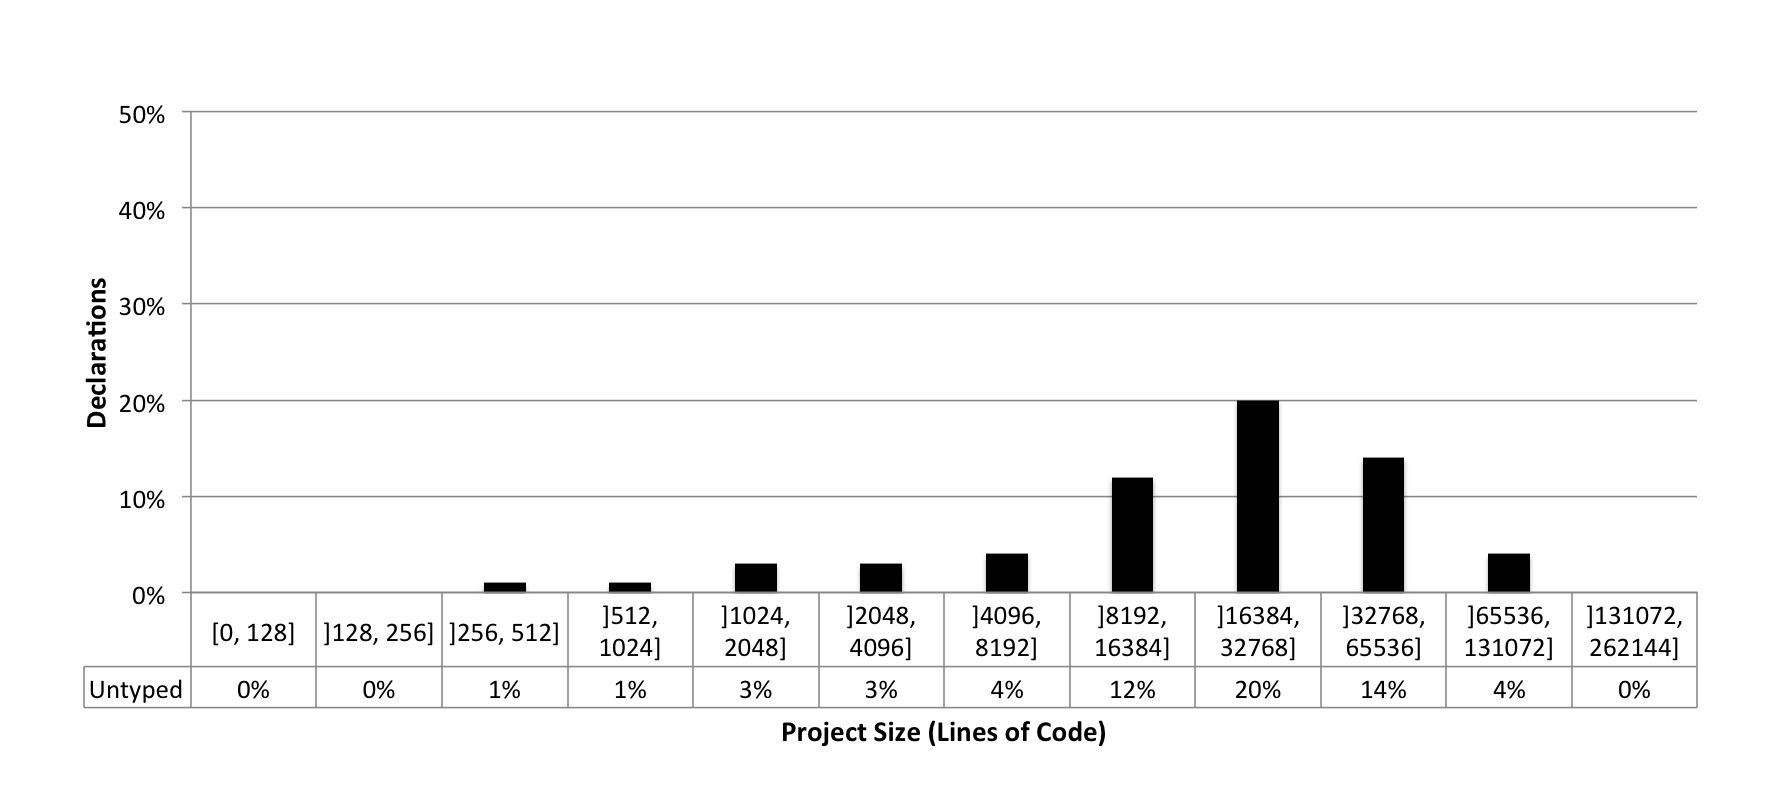
\includegraphics[width=1\textwidth]{images/size_proMethodReturn} 
\caption{Dynamic Typing usage in local variables}
\label{fig:size_proMethodReturn} 
\end{figure*}

Conversely, the use of untyped declarations in local variables increases with the project size. 
This is shown in figure \ref{fig:size_localVariable}. 
The average frequency of untyped local variable declarations in projects with less than $512$ lines of code is less than $40\%$. 
On the other side, in projects with over $65536$ lines of code, the average frequency for this type of declaration exceeds $70\%$.

\begin{figure*}[ht]
\centering 
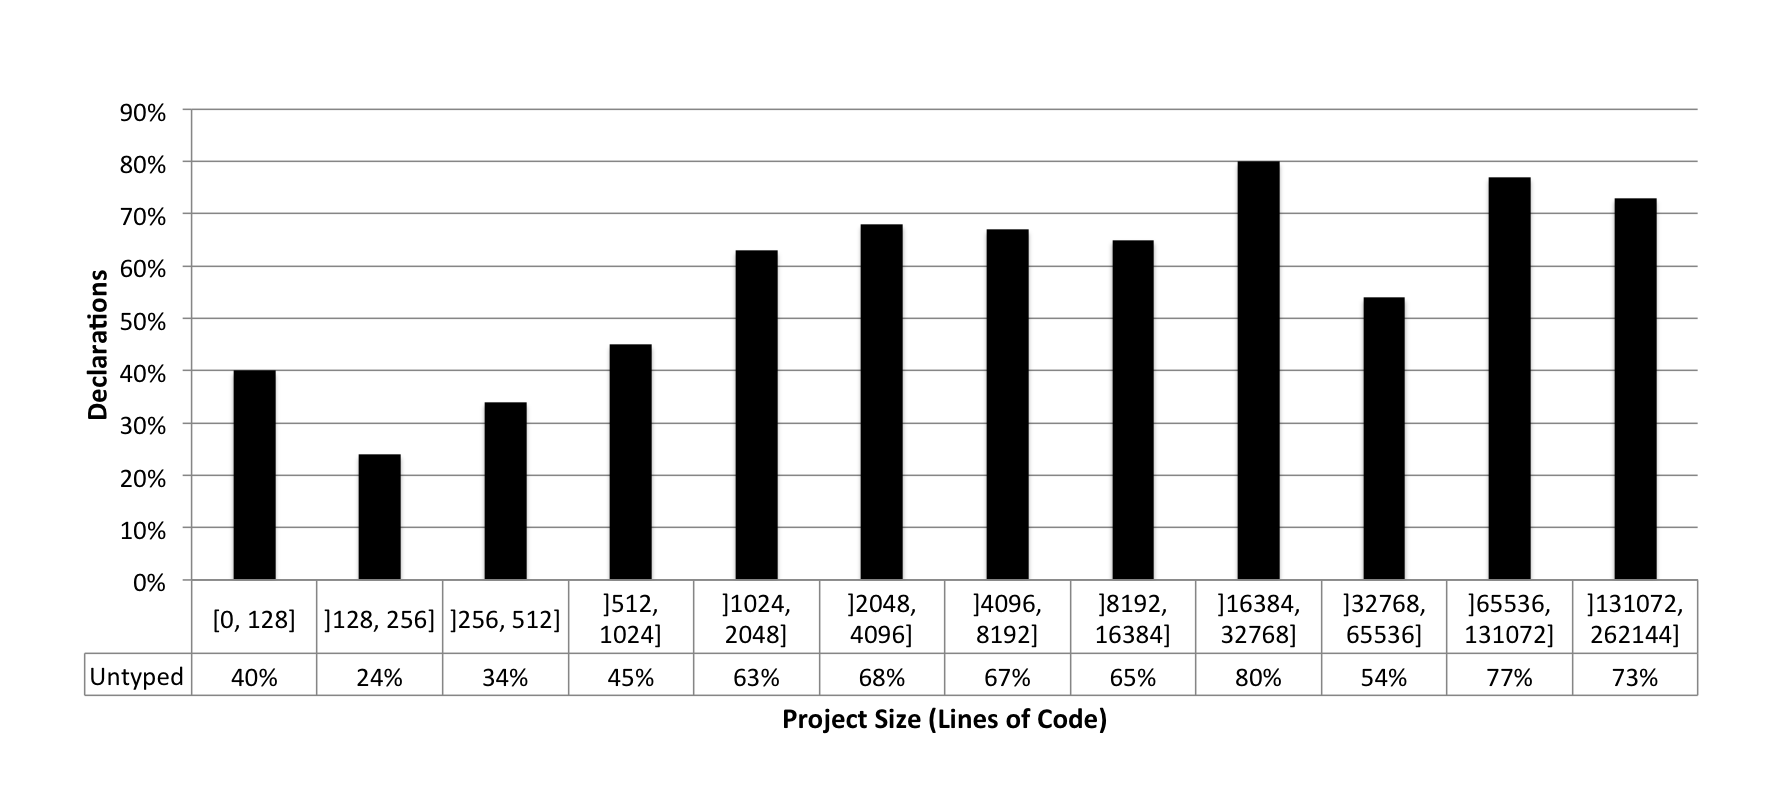
\includegraphics[width=1\textwidth]{images/size_localVariable} 
\caption{Dynamic Typing usage in local variables}
\label{fig:size_localVariable} 
\end{figure*}

TODO: Here I will add some text to explain the spearman ranking of these variables.

\begin{table}[ht]
\caption{Spearman Ranking for Dynamic Typing Usage over Size}


\centering{}%
\begin{tabular}{|rr|c|}
\hline 
\multirow{3}{*}{Method Return}			& public 			& ?\\
									& private 			& ?\\
									& protected		& ?\\
\hline
\multirow{3}{*}{Method Parameter}			& public 			& ?\\
									& private 			& ?\\
									& protected		& ?\\
\hline
\multirow{3}{*}{Constructor Parameter}		& public			& ?\\
									& private 			& ?\\
									& protected		& ?\\
\hline
\multirow{3}{*}{Field}					& public 			& ?\\
									& private 			& ?\\
									& protected		& ?\\
\hline
									& Local Variable	& ?\\
\hline  	
\end{tabular}
\label{tab:size_dynamic_spearman}
\end{table}



\subsection{Scripts\label{sub:scripts}}
Table \ref{tab:scritps} shows that the usage of types in scripts is not significantly different form the overall usage shown in section \ref{sub:overall-result}.

\begin{table}[ht]
\caption{Type System used in different contexts}


\centering{}%
\begin{tabular}{|c|c|c|}
\hline 
 & Static Typing & Dynamic Typing\tabularnewline
\hline 
\hline 
Scripts & 63\% & 37\%\tabularnewline
\hline 
Classes & 60\% & 40\%\tabularnewline
\hline 
\end{tabular}
\label{tab:scritps}
\end{table}


\subsection{Test Classes\label{sub:scripts}}

There is a slight difference between the definition of types in tests classes and all other classes. This is shown in table \ref{tab:tests}

\begin{table}[ht]
\caption{Type System used in different contexts}
\centering{}%
\begin{tabular}{|c|c|c|}
\hline 
 & Static Typing & Dynamic Typing\tabularnewline
\hline  
\hline 
Test Classes & 56\% & 44\%\tabularnewline
\hline 
Other Classes & 68\% & 32\%\tabularnewline
\hline 
\end{tabular}
\label{tab:tests}
\end{table}


\section{Discussion\label{sec:Discussion}}

In this section we build on the results presented in section \ref{sec:Resultados} to discuss what are the factors that we find to be influencing the choice for a static type system.

TODO Please, don't review this sextion yet. It's still not clear to me how to put together Results and Discussion section. I wanna discuss this a little more before I move on. 

\subsection{Previous experience of developers\label{sub:previous_experience}}
Section \ref{sub:overall-result} shows that about 61\% of the statements are typed. 
This results show that, even though Groovy is a dynamic language, Groovy programmers prefer the convenience of typed declarations most of time.
Groovy is a popular language among Java developers.
Assuming that a significant part of these Groovy developers had some previous experience with Java and were use to static typing, this suggests that the previous experience of a programmer is an important factor in choosing the type system.

TODO This section is really weak without solid data that indicates that these developers have some experience with Java. I suggest getting the fraction of developers who also have Java projects in GitHub. Maybe we even could show the results above grouped by developers who have Java projects and other developers.

\subsection{Scope and life cycle\label{sub:scope_lifecycle}}
Scope and life cycle seem to be 

Figure \ref{fig:tipo_declaracao} shows that dynamic typing is used in local variables declarations with more frequency than in other types of statements.
Since local variables have smaller scope and shorter life time, programmers probably feel less need to document them through the definition of types and end up choosing a simpler way to declare them, by using dynamic typing.

Conversely, constructor parameters are the declaration type with the most static typing usage.
It can be argued that there is a relevant concern in documenting these statements by the usage of static typing since these are important elements in the definition of the contract of a module.

\subsection{Results by Visibility\label{sub:visibility-results}}
According to figure \ref{fig:method_return_visibility}, statements with public or protected visibility are those more frequently statically typed. 
These statements define the interface of a module and, by typing them, programmers allow the compiler to look for typing problems in the integration with other modules.
In addition to that these statements should be well documented so clients of this module know how to use it making static typing a good option for that purpose.

In the case of parameters and returns of methods, the usage of types in statements with protected visibility even surpasses that of statements with public visibility.
It can be argued that protected fields and methods establish a tight contract, since they expose internal elements of a superclass to a subclass.
Apparently programmers understand that this type of contract should be well document to avoid any problems in such a delicate context.

\subsection{Results by Project Size\label{sub:size-results}}
Figure \ref{fig:size_pubMethodReturn} shows the use of dynamic typing in public statements by project size. 
Each bar of this graph show the result for projects grouped by their size.
The boundaries of each group are defined under each bar.
For example, a project with $1500$ lines of code is in the second group, since $1500$ lies within the interval $]400, 1600]$.

This result shows that the use of dynamic typing in public statements decreases as the size of the project
increases. 
The frequency of dynamic typing usage in projects with more than 6400 lines of code is almost half the frequency of smaller projects.
Intuitively, the larger the project, the greater the difficulty of integration and the need for maintenance.
This may lead programmers to prefer the use of static typing in public statements, the most critical  statements in this context.
No pattern can be observed in other types of statements, reinforcing the idea that this behavior is related to the role of public elements in large projects.

\subsection{Scripts e Testes\label{sub:Scripts-e-Testes}}
Scripts are usually written to perform simple tasks and do not relate to many other modules. 
The same can be said for test code. 
This suggests that dynamic typing would be used more often in such contexts since maintainability and integration are not critical factors for tests or scripts. 
The result shown in table \ref{tab:teste} however contradicts this idea.
There is no significant difference in the usage of typing systems in these contexts.


\section{Threats to Validity\label{sec:ameaca}}
As mentioned in section \ref{sub:overall-result}, programmers tend to continue using the type system they are used to.
Given that most Groovy programmers have prior experience with Java, a statically typed language, the results shown in this work might present a certain tendency to favor static type systems. 
Nevertheless, the analysis by type of declaration given in section \ref{sub:declaration-type-results} shows the predominance of dynamic typing over local variable declarations, indicating that, despite the previous experience with Java,
programmers are able to learn to use dynamic typing where they consider it necessary.

Some frameworks require the use of a particular type system in certain situations. 
Spock, for example, a automated testing framework, requires that the return of test methods to be dynamically typed. 
However, due to the heterogeneity and the large number of projects analyzed, we believe that there is no framework capable of having a significant influence on the overall results of this study.

\section{Related Work\label{sec:Trabalhos-Relacionados}}
There are some works in the literature that compare static and dynamic typing systems though controlled studies.
In \cite{experiment_with_purity}, the author compares the performance of two groups of students when asked to develop two small systems. 
Both groups used a language developed by the author, Purity. 
The only difference in the language used by the two groups was the typing system.
One group used a statically typed version of Purity while the other used a dynamically typed version of the same language.
Results showed that the group using the dynamic version was significantly more productive than the other. 
Similarly to this work, the author was able to compare two type systems directly while isolating any external factors. 
However, it can be argued that these results may not represent well real life situations of the software industry. 
This was a short duration study where students were used as examples of developers with no interaction with other programmers. 
In this paper, we try to get more relevant results when analyzing source code developed by programmers during their normal activities.

In a follow up study \cite{hanenberg_icpc}, the authors got to opposite conclusions. 
They compared the performance of two groups of developers in maintenance tasks. 
First group used Java, a statically typed language, and the other used Groovy, but restricting developer to use only dynamic typing in order to simulate a dynamically typed Java.
In this case, the group using the statically typed language, Java, was much more productive.
This contradiction reinforces the argument that the results of controlled studies aren't reliable enough for this type of study.

In experiments conducted in \cite{ruby_vs_druby}, the authors compare the performance of two groups working on small development tasks.
One group used Ruby, a dynamically typed language, while the other used DRuby, a statically typed version of Ruby. 
Results showed that the DRuby compiler rarely managed to capture any errors that weren't already evident for programmers.
Most subjects involved in the study had previous experience with Ruby, which suggests that programmers get used to the lack of static typing in their declarations.

\section{Conclusions and Future Work\label{sec:Conclus=0000E3o-e-Trabalhos}}
This study examines what are the most influencing factors in the choice for a static or dynamic type system. 
There are some controlled studies in the literature about the advantages of each one of these typing system already. 
However the results presented here focus on finding the factors that have an actual influence on the decision for one or another through the analysis of a wide range of source code repositories.

When maintainability and the complexity of the integration between modules are considered important, static typing is apparently preferred by Groovy programmers. 
In these situations, the advantages of static typing such as documenting the code or integrating with software development tools, are relevant advantages considered by Groovy programmers.
Conversely, when these issues are not as critical, the simplicity of dynamic typing seems to be preferred, as seen on local variables declarations.
Another important factor is the previous experience of programmers with a given type system.

In future works we wish to analyze the influence of static and dynamic type systems over the robustness of software systems.
In particular , we want to understand whether the use of dynamic typing, which limits the compiler's ability to find type problems, has any correlation with the occurrence of defects in the system and if the use of automated testing is able to reduce this correlation.

\acks
This work was partially supported by FAPEMIG, grants APQ-02376-11 e APQ-02532-12, and CNPq grant 485235/2011-0. 

% We recommend abbrvnat bibliography style.

\bibliographystyle{abbrvnat}

% The bibliography should be embedded for final submission.

\begin{thebibliography}{}
\softraggedright

\bibitem[Tiobe Website(2013)]{tiobe}
Tiobe programming community index. http://www.tiobe.com/index.php/ content/paperinfo/tpci/index.html. Accessed in 23/06/2013.

\bibitem[Bruce, K. (2002)]{bruce2002foundations}
Bruce, K. (2002). Foundations of object-oriented languages: types and semantics. MIT press.

\bibitem[Bruch, M., Monperrus, M., and Mezini, M. (2009)]{bruch2009learning}
Bruch, M., Monperrus, M., and Mezini, M. (2009). Learning from examples to improve code completion systems. In Proceedings of the the 7th joint meeting of the European software engineering conference and the ACM SIGSOFT symposium on The foundati- ons of software engineering, pages 213–222. ACM.

\bibitem[Cardelli, L. (1996]{type_systems}
Cardelli, L. (1996). Type systems. ACM Comput. Surv., 28(1):263–264.

\bibitem[Chang, M., Mathiske, B., Smith, E., Chaudhuri, A., Gal, A., Bebenita, M., Wimmer, C.]{jit}
Chang, M., Mathiske, B., Smith, E., Chaudhuri, A., Gal, A., Bebenita, M., Wimmer, C., and Franz, M. (2011). The impact of optional type information on jit compilation of dynamically typed languages. SIGPLAN Not., 47(2):13–24.

\bibitem[Daly, M. T., Sazawal, V., and Foster, J. S. (2009)]{ruby_vs_druby}
Daly, M. T., Sazawal, V., and Foster, J. S. (2009). Work In Progress: an Empirical Study of Static Typing in Ruby. In Workshop on Evaluation and Usability of Programming Languages and Tools (PLATEAU), Orlando, Florida.

\bibitem[Hanenberg, S. (2010)]{experiment_with_purity}
Hanenberg, S. (2010). An experiment about static and dynamic type systems: doubts about the positive impact of static type systems on development time. SIGPLAN Not., 45(10):22–35.

\bibitem[Kleinschmager, S., Hanenberg, S., Robbes, R., and Stefik, A. (2012)]{hanenberg_icpc}
Kleinschmager, S., Hanenberg, S., Robbes, R., and Stefik, A. (2012). Do static type systems improve the maintainability of software systems? An empirical study. 2012 20th IEEE International Conference on Program Comprehension (ICPC), pages 153– 162.

\bibitem[Lamport, L. and Paulson, L. C. (1999)]{should_your_specification_language_be_typed}
Lamport, L. and Paulson, L. C. (1999). Should your specification language be typed. ACM Trans. Program. Lang. Syst., 21(3):502–526.

\bibitem[Mayer,C.,Hanenberg,S.,Robbes,R.,Tanter,E ́.,andStefik,A.(2012)]{mayer2012static}
Mayer,C.,Hanenberg,S.,Robbes,R.,Tanter,E ́.,andStefik,A.(2012).Statictypesys- tems (sometimes) have a positive impact on the usability of undocumented software: An empirical evaluation. self, 18:5.

\bibitem[Pierce, B. (2002)]{types_and_programming_languages}
Pierce, B. (2002). Types and programming languages. MIT press.

\bibitem[Tratt, L. (2009)]{dynamically_typed_languages}
Tratt, L. (2009). Chapter 5 dynamically typed languages. volume 77 of Advances in Computers, pages 149 – 184. Elsevier.

\bibitem[Siek, Jeremy, and Walid Taha(2007)]{gradual_typing}
Siek, Jeremy, and Walid Taha. "Gradual typing for objects." ECOOP 2007–Object-Oriented Programming. Springer Berlin Heidelberg, 2007. 2-27.

\bibitem[Gray(2008)]{gray08}
GRAY, K. E. Safe cross-language inheritance. In European Conference on Object-Oriented Programming (2008), pp. 52–75.

\bibitem[Gray(2011)]{gray11}
GRAY, K. E. Interoperability in a scripted world: Putting inheritance \& prototypes together. In Foundations of Object-Oriented Languages (2011).

\bibitem[Gray(2005)]{gray05}
GRAY, K. E., FINDLER, R. B.,ANDFLATT, M. Fine-grained interoperability through contracts and mirrors. InObject-Oriented Programming, Systems, Languages, and Applications(2005), pp. 231–245.

\bibitem[Siek(2007)]{siek07}
SIEK, J.,ANDTAHA, W. Gradual typing for objects. In European Conference on Object-Oriented Programming(2007),pp. 2–27.

\bibitem[Takikawa(2012)]{takikawa12}
Takikawa, Asumu, et al. "Gradual typing for first-class classes." ACM SIGPLAN Notices. Vol. 47. No. 10. ACM, 2012.

\end{thebibliography}


\end{document}

%                       Revision History
%                       -------- -------
%  Date         Person  Ver.    Change
%  ----         ------  ----    ------

%  2013.06.29   TU      0.1--4  comments on permission/copyright notices

